\begin{center}
\Huge
Ligningen for en tangent.
\end{center}
\section*{Hvordan vi finder ligningen for tangenten i et punkt}
\stepcounter{section}


Hvis vi har en differentiabel funktion $f$, så kan vi bestemme hældningen af funktionen i punktet $x_0$ ved at bestemme $f'(x_0).$
Vi vil gerne kunne bestemme ikke blot tangentens hældning i dette punkt, men hele ligningen for tangenten. Vi betragter følgende algoritme:
\begin{enumerate}[label=\roman*)]
	\item Vi skal finde en ligning for tangenten på formen $y=ax+b$. 
	\item Vi ved, at hældningen skal være $a = f'(x_0)$, så vi bestemmer $f'$ og evaluerer den i $x_0$.
	\item Vi ved, at ligningen for tangenten skal gå igennem punktet $(x_0,f(x_0))$, så vi bestemmer $f(x_0)$ og løser ligningen 
	\begin{align*}
		\underbrace{f(x_0)}_{=y_0} = \underbrace{f'(x_0)}_{=a}x_0 + b\ \Leftrightarrow\ b = f(x_0) - f'(x_0)x_0.
	\end{align*}
	\item Vi har nu bestemt tangentens ligning $y = ax + b$.
\end{enumerate}
Vi kan samle denne algoritme til en sætning:
\begin{setn}[Tangentens ligning]
	Lad $f$ være en differentiabel funktion i $x_0$. Så er ligningen for tangenten til $f$ i punktet $(x_0,f(x_0))$ givet ved
	\begin{align*}
		y = f'(x_0)(x-x_0) + f(x_0).
	\end{align*}
\end{setn}
\begin{proof}
	Da $a = f'(x_0)$ og $b =  f(x_0) - f'(x_0)x_0$ fås 
	\begin{align*}
		y = ax+b = f'(x_0)x + f(x_0)-f'(x_0)x_0 = f'(x_0)(x-x_0) + f(x_0).
	\end{align*}
\end{proof}
\begin{exa}
Vi ønsker at finde ligningen for tangenten til funktionen $x^2$ i punktet $(1,1)$. Vi finder først den afledede til $x^2$:
\begin{align*}
(x^2)' = 2x.
\end{align*}
Derfor må hældningen af tangenten i punktet $(1,1)$ være $a = f'(1) = 2$. Vi skal nu finde $b$ i ligningen $y=2x+b$, så vi indsætter vores kendte punkt:
\begin{align*}
y = 2x+b \Leftrightarrow 1= 2\cdot 1 +b \Leftrightarrow b = -1,
\end{align*}
og derfor må tangentens ligning i punktet $(1,1)$ være givet som
\begin{align*}
y = 2x-1.
\end{align*}
Funktionen $x^2$ og tangenten i punktet $(1,1)$ til $x^2$ fremgår af Fig. \ref{fig:tangent}.

\begin{figure}[H]
	\centering
	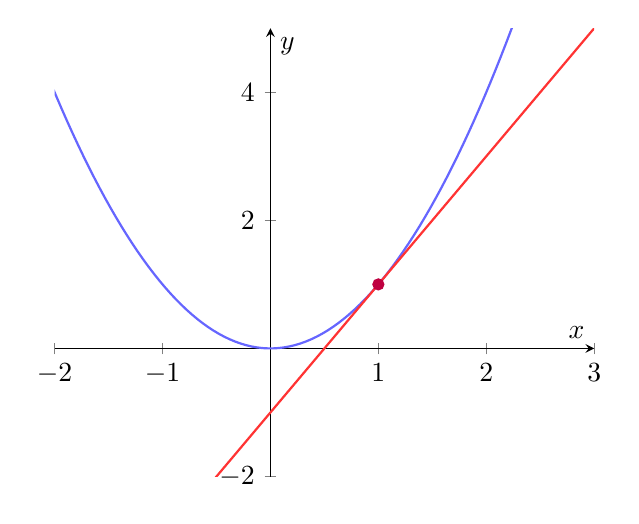
\begin{tikzpicture}
		\begin{axis}[
		axis lines = middle, 
		xmin = -2, xmax = 3, 
		ymin = -2, ymax = 5,
		xlabel = {$x$},
		ylabel = {$y$}
		]
			\addplot[color = blue!60, samples = 200,thick] {x^2};
			\addplot[color = red!80, samples = 200,thick] {2*x-1};
			\filldraw[color = purple] (axis cs:1,1) circle (2pt); 
		\end{axis}
	\end{tikzpicture}
	\caption{Funktion $f(x)=x^2$ og tangentlinjen $g(x) = 2x-1$.}
	\label{fig:tangent}
\end{figure}
\end{exa}

\begin{setn}
Funktionen $f(x)=x^3$ er overalt differentiabel med differentialkvotient
\begin{align*}
\frac{d}{dx}x^3 = (x^3)' = 3x^2. 
\end{align*}
\end{setn}
\begin{proof}
Vi anvender definitionen af differentialkvotienten:
\begin{align*}
f'(x) = \lim_{h\to 0}\frac{f(x+h)-f(x)}{h},
\end{align*}
hvilket i tilfældet $f(x) = x^2$ giver
\begin{align*}
(x^3)' &= \lim_{h\to 0}\frac{(x+h)^3-x^3}{h}\\
&= \lim_{h\to 0} \frac{(x^2+h^2+2xh)(x+h)-x^2}{h}\\
&= \lim_{h\to 0} \frac{x^3+xh^2+2x^2h+x^2h+h^3+2xh^2-x^3}{h}\\
&= \lim_{h\to 0} \frac{xh^2+2x^2h+x^2h+h^3+2xh^2}{h}\\
&= \lim_{h\to 0} xh+2x^2+x^2+h^2+2xh\\
&= \lim_{h\to 0} 3x^2+3xh+h^2\\
&= 3x^2.
\end{align*}
\end{proof}

\section*{Opgave 1}
Find ligningen for tangenten til følgende funktioner i de tilhørende punkter. Tegn desuden funktionerne og tangentlinjerne i Maple for at undersøge, om du har fundet de rigtige tangentlinjer. 
\begin{align*}
&1) \ f(x) = x^2,\  P(-1,f(-1))  &&2) \   f(x)=2x^2-1x+3, \ P(0,f(0))    \\
&3) \ f(x) = \frac{1}{x} -x^3, \ P(2,f(2))   &&4) \ f(x) = \sqrt{x}, \ P(4,f(4))    \\
&5) \ f(x) = 7x+3,\ P(3,f(3))   &&6) \ f(x) = -3x^2+5x-1, \ P(1,f(1))     \\
&7) \ f(x) = 27, \ P(1000,f(1000))   &&8) \ f(x) = 3x^2-2\sqrt{x}, \ P(9,f(9))     \\
&9) \ f(x) = \frac{10}{x}+3x^3, \ P(2,f(2))   &&10) \ f(x) = 5x^3+2x^2+x+1, \ P(-2,f(-2))     \\
\end{align*}
